\documentclass{article}


%\usepackage{times}
%If you have times installed on your system, please
%uncomment the line above

%For figures and tables to stretch across two columns
%use \begin{figure*} \end{figure*} and
%\begin{table*}\end{table*}
% please place figures & tables as close as possible
% to text references
\usepackage{natbib}
\usepackage{amsfonts}
\usepackage{amsmath}
\usepackage[usenames]{color}
\usepackage{ulem}
\usepackage{verbatim}
\usepackage{longtable}
\usepackage{array}
\usepackage{epsfig}
\usepackage{graphicx}
\usepackage{threeparttable}
\usepackage{epstopdf}


\newcommand{\be}{\begin{equation}}
\newcommand{\ee}{\end{equation}}
\citestyle{apj}
\newcommand{\todo}[1]{{\color{blue}$\blacksquare$~\textsf{[TODO: #1]}}}
\newcommand{\todored}[1]{{\color{red}$\blacksquare$~\textsf{[TODO: #1]}}}
\newcommand\msun{M$_\odot$}
\newcommand\lsun{L$_\odot$}
\newcommand\mzams{$M_{\rm ZAMS}$}
\newcommand\pasa{PASA}
\newcommand\rh{R$_{\rm h}$}



\title{Bayesian Non-Parametric Modeling of Extragalactic Globular Cluster Populations}

\author{Zachary G. Jennings}

\begin{document}
\maketitle

\begin{abstract}
I apply Bayesian semi-parametric density estimation methods to the bivariate color-color distributions of
extragalactic globular cluster systems. I implement a blocked Gibbs sampler that treats these distributions
as Dirichlet process mixtures of multivariate normals. I also implement a simple mode finding algorithm to
infer the number of distinct modes in realizations of the underlying functional distribution for the density.
I apply this method to GC datasets for two galaxies, NGC 3115 and NGC 4494. NGC 3115 displays very clear bimodality,
confirming the traditional paradigm of two underlying and distinct GC populations for this galaxy. This suggests that
NGC 3115 has undergone two distinct formation epochs in its history. However, NGC 4494 appears to be better-modeled
by a unimodal density, suggesting a single formation epoch or perhaps a more continuous process of assembly over
its lifetime. I briefly note potential extensions of the model, and other potential inferences of interest which could
be measured from the posterior distributions of the density function.
\end{abstract}

\section{INTRODUCTION}
Globular Clusters (GCs) are tightly bound clusters of $\sim10^5$ stars packed into regions just a few
parsecs on radius. They live in the outer dark matter halos of galaxies and are among the oldest and densest
stellar populations in the universe. GCs are noteworthy not just for their exotic internal properties; indeed, this extreme
stellar density can only be achieved in especially intense events of star formation, and this density allows GCs to remain
gravitationally bound during galaxy merger events which will destroy less bound clusters. The GC population
of a given galaxy can be thought of as a sort of archeological record of that galaxy's assembly history. GCs will
either be created in the largest star formation events early in a galaxy's lifetime or deposited in the halo through mergers
with other galaxies. See \citealt{brodie2006} for an extensive review of extragalactic GC systems.

Given the role GCs play in tracking the assembly history of a galaxy, understanding any subpopulations in the various
distributions of GCs around galaxies can give us a window into the relative importance of different assembly periods
in a galaxy's life. \citealt{zepf1993} first noted in (at the time) high-precision photometry that GC distributions
appear to be bimodal in color, with distinct red and blue subpopulations. Over the past couple decades, the bimodality
of GC systems has been verified to be a common feature in many different populations, and has become interpreted
as a necessary observation that any theory of GC formation must match. 

Astronomers define a "color" as the difference between the logs of fluxes measured in two
separate broadband filters. For example, the color $g-i$ is defined $(g-i)=\log(F_g/F_i)$. Bimodality in color
is interesting because it corresponds to bimodality in chemical composition. To first order, the color of a star of a given
mass is determined by the presence of heavy elements in the stellar atmosphere. The more heavy elements, the
cooler the star is for a given mass, and therefore the more red it is. When we analyze the full integrated light of
all the stars in this globular cluster, the color of this light is a very good proxy to the average chemical composition
of stars in the cluster. All these statements are quite well-established in fundamental astrophysics, and the color
distributions of systems of GCs can be thought of as a strong measurement of the heavy element composition distribution
of a GC system.

Elemental composition is interesting specifically because it corresponds to the material which went in to making the stars
in the first place. Stars which are more enriched in heavier elements have been born out of material which has been already
polluted by previous generations of stars, meaning these stars were born later in the universe. A unique population of GCs
in a galaxy indicates a specific formation epoch in a galaxy, and the number of these epochs can be an important constraint
on how a given galaxy has evolved over its lifetime. As a result, even if it seems a somewhat simple question, understanding
how many populations of GCs there are in a galaxy and the properties of each of these populations offers a powerful
window into understanding galaxy evolution in a broader cosmological context.

\section{DATA AND MODEL}
Typically, the color-color distributions of extragalactic GC systems are parameterized as
finite mixture models of two multivariate normal distributions. There is no real physical motivation
for such a mixture, but it does offer a convenient parameterization that allows conjugate priors to be specified
for ease of computation. For however many $n+1$ filters we have used for our imaging, we will
have $n$ independent color measurements. For most cases, we acquire three-filter photometry of our extragalactic
GC systems, leading to a bivariate dataset, which is what I will consider in this paper.

The full model specification is as follows: 
\begin{eqnarray}
y_i \sim \rm{MVN}(\mu_i,\Sigma) \\
\mu_i | G \stackrel{iid}{\sim}G,\\
G | \alpha,\psi \sim DP(\alpha,G_0(.|\psi_1,\psi_2)), \\
\Sigma,\alpha,\psi_1,\psi_2 \sim p(\Sigma)p(\alpha)p(\psi_1)p(\psi_2)\\
p(\psi_1) \sim MVN (a_{\psi_1},b_{\psi_1},\\
p(\psi_2) \sim W^{-1}(a_{\psi_2},b_{\psi_2}),\\
p(\Sigma) \sim W^{-1}(a_{\Sigma},b_{\Sigma}),\\
p(\alpha) \sim \rm{Gamma}(a_\alpha,b_\alpha).
\end{eqnarray}

The choice of a multivariate normal for the $G_0$ function is a convenient parameterization for the problem of interest.
As we discussed in class, the precise choice for this function probably isn't too important so long as the support is correct,
and I found a MVN worked well. The conjugate priors for the $\psi$ parameters are another multivariate normal
for the mean, and an inverse Wishart distribution for the covariance matrix, both of which have their own hyperparameters
to specify. I also used an inverse Wishart distribution for the kernel covariance $\Sigma$, and finally a Gamma prior
on $\alpha$ for updating using the data augmentation strategy.

In principle $\Sigma$ can be indexed to $\Sigma_i$ to allow each kernel to have its own covariance matrix,
and in fact I coded a version of the model with this option. However, I found the computation time for this
model extremely slow. I imagine this is mostly due to poor optimization on my part; steps took many times longer
than they did when $\Sigma$ was shared across models. While a $\Sigma_i$ that is allowed to vary is going to allow the model
more flexibility and is probably the most powerful implementation, for purposes of this class project, I decided
the single $\Sigma$ was sufficient. Better-optimized code could almost certainly be written to alleviate the computational
difficulty.

\section{METHODS}
To perform density estimation, I implemented the blocked Gibbs sampler as described in \citealt{ishwaran2001}:

\begin{eqnarray}
y_i | Z,L_i, \Sigma \stackrel{ind}{\sim} \rm{MVN}(y_i | \mu_i,\Sigma) \\
L_i | p \stackrel{iid}\sim \sum^{N}_{l=1}p_l\delta_l(L_i),\\
Z_l | \psi \stackrel{iid}\sim MVN(. | \psi_1,\psi_2), \\
p | \alpha \sim f(p,\alpha),\\
\Sigma,\alpha,\psi_1,\psi_2 \sim p(\Sigma)p(\alpha)p(\psi_1)p(\psi_2),\\
p(\psi_1) \sim MVN (a_{\psi_1},b_{\psi_1},\\
p(\psi_2) \sim W^{-1}(a_{\psi_2},b_{\psi_2}),\\
p(\Sigma) \sim W^{-1}(a_{\Sigma},b_{\Sigma}),\\
p(\alpha) \sim \rm{Gamma}(a_\alpha,b_\alpha).
\end{eqnarray}

I won't reproduce the full algorithm here, since it just comes from the notes, but essentially all the updates are just
straightforward Gibbs samplings. When drawing values for $Z_i$, we draw for values which have currently been
assigned to data from $G_0$ times the likelihood of the kernel for those data. Otherwise we draw new values.
The $p$ array is just updated sequentially using the stick breaking construction, and then the $L_i$ are just drawn
from these discrete distributions. Updates on the $\psi$ and $\Sigma$ parameters are just draws from MVN and Inverse
Wishart distributions given the conjugacy of prior specification, and the $\alpha$ updates are draws from a Gamma when
a Gamma prior is assumed.

This model essentially replicates the functionality of the \texttt{DPdensity} package in \texttt{R}, but
I decided to write a from-scratch implementation in Python as this has become the de-facto computer
language in Astronomy. My code makes use of nothing other than the standard \texttt{numpy} and
\texttt{scipy} libraries, and so should be quite generally applicable for applications where it is preferable to have
code in Python.

Our primary research question is to understand the shape and uncertainty in the underlying distribution for the density,
$G$. It is here that the non-parametric Bayesian approach is so powerful. While simple non-parametric
density estimation in this context
is a fairly straightforward process, the Bayesian approach is fundamentally probabilistic and can therefore provide us
an estimate of uncertainty on the underlying functional. For the blocked Gibbs sampler, this inference comes "for free"
in the course of doing our MCMC samples. The stick breaking construction for each iteration of the sampler manifests
as a vector of $p$ values which essentially represent the relative strength of each kernel at that point in a model.
We can define a grid over data locations where we evaluate the density of the model at each point for a single
run of the chain. The mean functional is then just the average of these values, and the range of the value of the PDF
at each point gives us a bound on the uncertainty. 

While there are further questions that could be pursued, one of the first values of interest for inference is the number of 
modes in the data. As we discussed in class, this is generally not going to be the same as considering inference on
$n_*$, the number of clusters in the data. Instead, I decided to use a mode finding scheme designed to select out
local minima and maxima in the data. I found a reasonably effective strategy was to apply both a maximum and minimum
filter to the mean functional, then define a difference grid where every point in this grid represents the difference between
the maximum and minimum. Any difference over a certain threshold can then be considered a local maximum.

The threshold value and the size of the filtering window are both parameters that need to be tuned for this method to work.
I examined different values for both when applied to some idealized mock datasets. Generally speaking, I found that
when one has some prior information about how far apart one expects modes to be, they can set the window to
a value appropriate for capturing this behavior. Once one does this, the precise specification of the threshold value
ends up not mattering too much. Applying this method to the mean functional gives us something of a point-estimate
for the number of populations in a given dataset, and applying it to each draw from the posterior of the functional
allows us to make a posterior distribution for the number of modes from the data.

%\section{TESTS ON IDEALIZED DATA}
%To test the inference of the model, I created some realizations of idealized data. In Fig.~\ref{fake_data},
%I plot one realization from a mixture of five multivariate normal distributions. Each of the multivariate normals
%has a covariance matrix
%$\Sigma = 
%\begin{pmatrix}
%0.25 & 0 \\
%0 & 0.25
%\end{pmatrix}
%$,
%but the mean vectors are allowed to be randomly selected anywhere between $[0,2]$. At this point, I run the model
%with prior parameters $a_{\Sigma}=4,b_{\Sigma}=\begin{pmatrix} 0.25 & 0.0 \\ 0.0 & 0.25\end{pmatrix},
%a_{\alpha}=1,b_{\alpha}=1,a_{\psi_1}=(1.0,1.0),b_{\Sigma}=\begin{pmatrix} 0.25 & 0.0 \\ 0.0 & 0.25\end{pmatrix}$.

\section{APPLICATION TO REAL DATA}
I applied the model to two globular cluster photometric datasets currently in the literature. These datasets both
involve imaging taken by our group using the SuprimeCam instrument on the 8m Subaru telescope on the summit
of Mauna Kea. Both datasets consist of imaging taken in three optical filters
(SDSS $g,r,~\textrm{and}~i$ for all three),
giving 2 independent color measurements for every GC in the dataset. I am sweeping a ton of details
involved preparing these datasets under the rug. The full problem requires one to also consider effects as to how
the globular clusters are selected; for purposes of the class project, I am assuming these datasets are perfectly selected.
For all plots of the data and distributions, I will plot the color index $(g-i)$ on the horizontal axis
and $(r-i)$ on the vertical axis.

The two galaxies, NGC 3115 and NGC 4494, are galaxies of similar size to the Milky Way, but with very different
morphologies. Both lack the spiral structure of our own galaxy, and instead can be thought of as ellipsoids of stars.
Such galaxies have likely had more active assembly histories than our own Milky Way, accreting many smaller galaxies
over the course of their lives. Such galaxies typically have richer GC systems than spiral galaxies like the Milky Way,
and as such the GC systems are particularly useful to study for these galaxies.

I assumed the same values for the hyperpriors for both datasets:

$a_{\Sigma}=4,b_{\Sigma}=\begin{pmatrix} 1.0 & 0.0 \\ 0.0 & 0.5\end{pmatrix},
a_{\alpha}=3,b_{\alpha}=1,a_{\psi_1}=(0.9,0.25),b_{\psi_1}=\begin{pmatrix} 0.5 & 0.0 \\ 0.0 & 0.3\end{pmatrix}$,

$a_{\psi_2}=5,b_{\psi_2} =\begin{pmatrix} 0.5 & 0.0 \\ 0.0 & 0.5\end{pmatrix}.$ In general, I found that precise specification of
hyperpriors for the $\psi$ parameters was very uninformative, as long as the locations were reasonably close
to the data and the variance allowed the blocked Gibbs sampler to look at reasonable regions of parameter space.
I found that while prior specification of $\alpha$ did have some affect on the values inferred for $\alpha$, $\alpha$
still seemed to learn from the data reasonably well, and the specification of $\alpha$ didn't have much effect on the
actually inferences on the full functional form of the data. However, as I discuss in the next section, it did seem
that the results were at least somewhat sensitive to the specification of the prior on the covariance matrix $\Sigma$.

\subsection{NGC3115 Photometry}
NGC3115 is a nearby galaxy located $\sim$10 Mpc away. The dataset I am using was published in \citealt{jennings2014},
and features around 650 total sources. NGC3115 is typically considered a textbook case in which the data are well-described
by a bimodal model, and it has been confirmed that the clear bimodality in color does in fact extend to a clear bimodality
in chemical composition as well, as expected \citep{brodie2012}.

I plot the color-color distribution of NGC3115 in Fig.~\ref{n3115_data}. I applied the model above and ran it for
3000 steps, discarding the first 1000, then thinned it by a factor of 5.
In Fig.~\ref{n3115_trace}, I plot traces for $\alpha$ and $n_*$, indicating that
the MCMC chain is reasonably well mixed. In Fig.~\ref{n3115_functional}, I plot the mean inference for 400 realizations
of $G$ from the blocked Gibbs sampler. The bimodal structure of $G$ is obvious in this plot. Finally, in Fig.~\ref{n3115_modes},
I plot the posterior for the number of modes found by my algorithm over the 400 realizations. I find the functional to be bimodal
in the vast majority of cases.

I found the results to be fairly dependent on the hyperpriors assumed for the inverse Wishart distribution on
the covariance matrix. I found that depending on the values given for the covariance in particular could have a big
influence on the final result. This effect was minimized somewhat by selecting parameters for the inverse Wishart
distribution which made it have a larger variance, but then the number of clusters in the model became very large
with smaller variances that were actually reasonable. I am also perhaps being unfair to $\Sigma$ by fixing
its hyperpriors and expecting it to find the solution as well as for the $\mu_i$ parameters, since $\Sigma$
naturally has less flexibility in how it may vary.

I think, with these data, I'm seeing a case where using a
single covariance matrix $\Sigma$ between the two cases ends up being a poor model. This is also supported by
a simple finite mixture model in which we assume two multivariate normals; I infer two fairly different matrices
for the two populations, with the redder GC distribution being more narrow. 

In any case, regardless of which prior is used for $\Sigma$, the underlying distribution tends to display two very
clear modes to the data. My mode finding algorithm confirms this, finding two modes in the underlying data in the
vast majority of cases. 

\begin{figure}
\centering
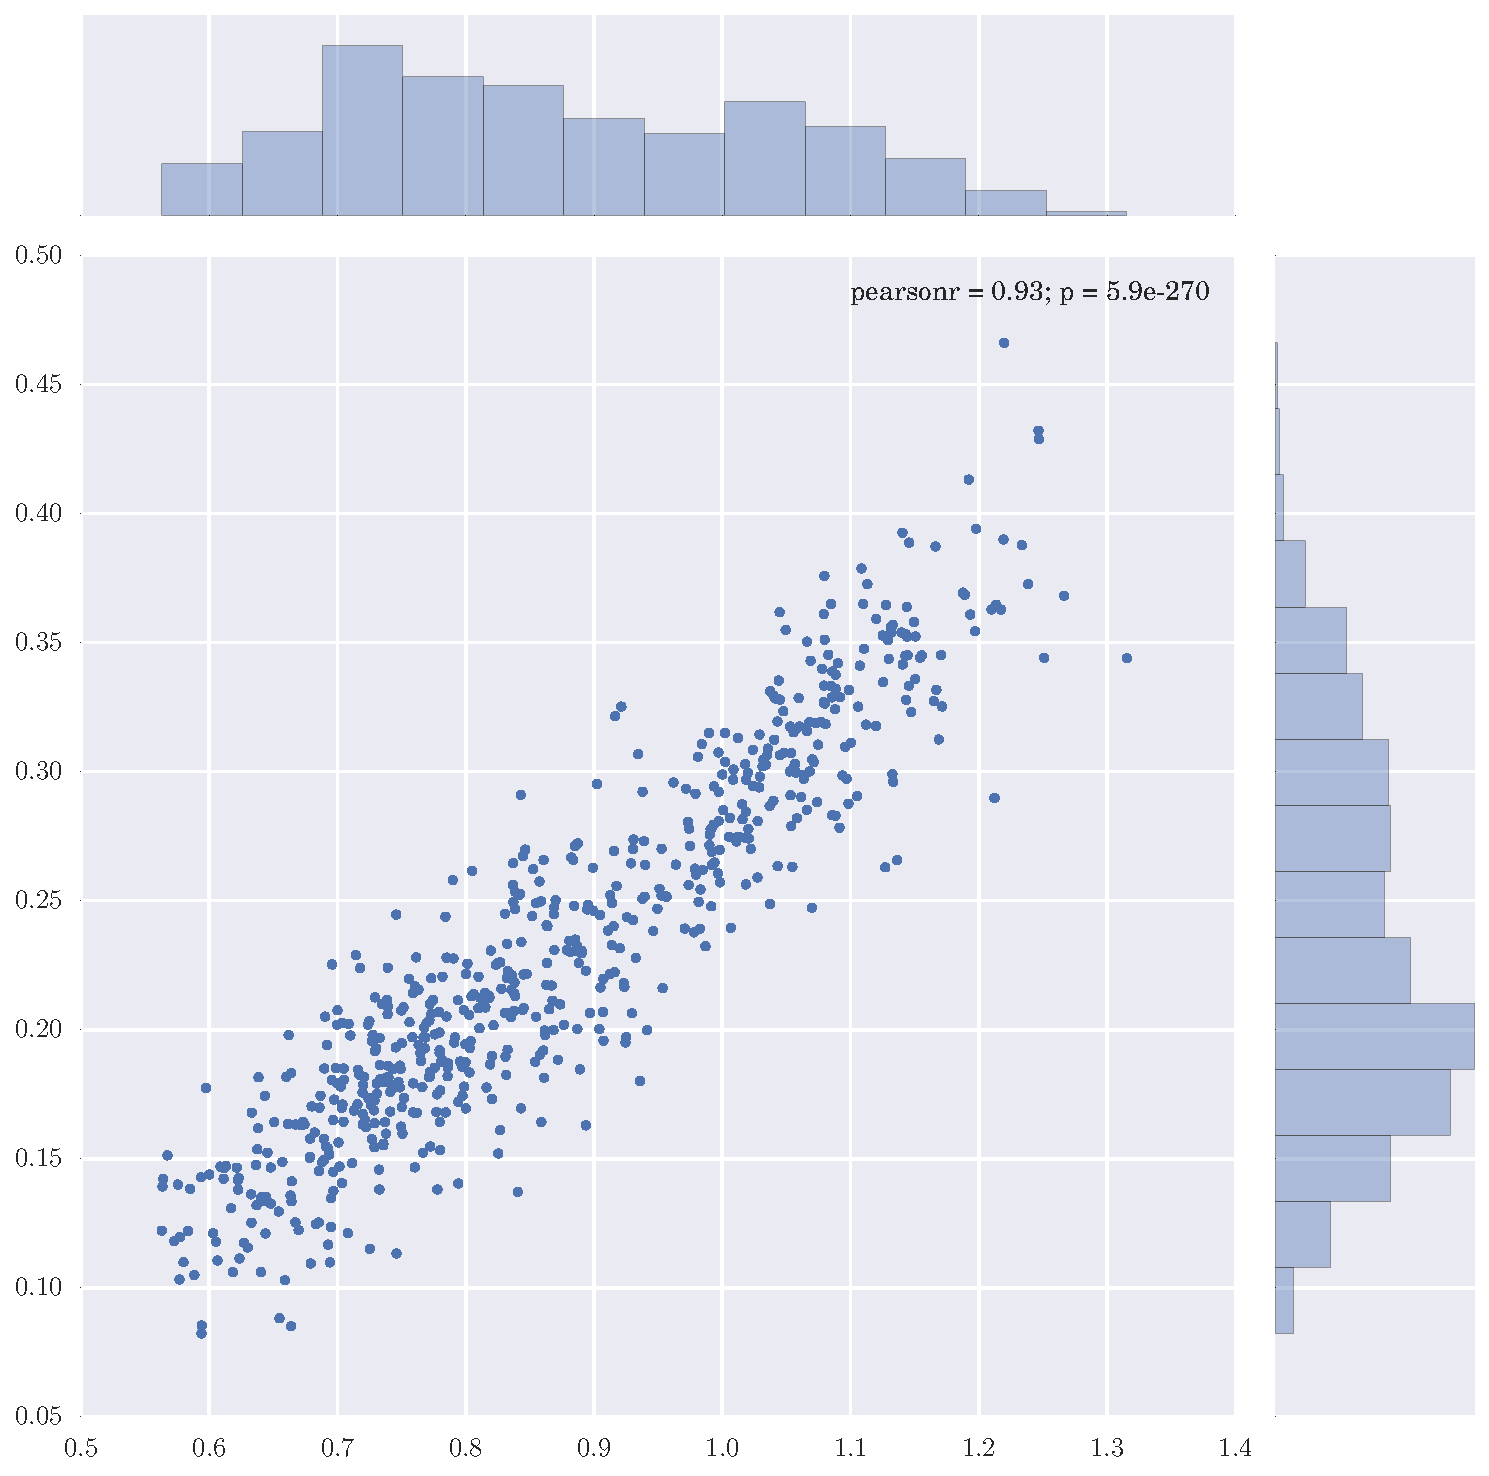
\includegraphics[width=0.6\textwidth]{n3115_data.pdf}
\caption{$(g-i)$ vs.~$(r-i)$ color-color plot of selected GCs around NGC 3115. Histogram at the top suggests a possible bimodal
structure in the underlying data.}
\label{n3115_data}
\end{figure}

\begin{figure}
\centering
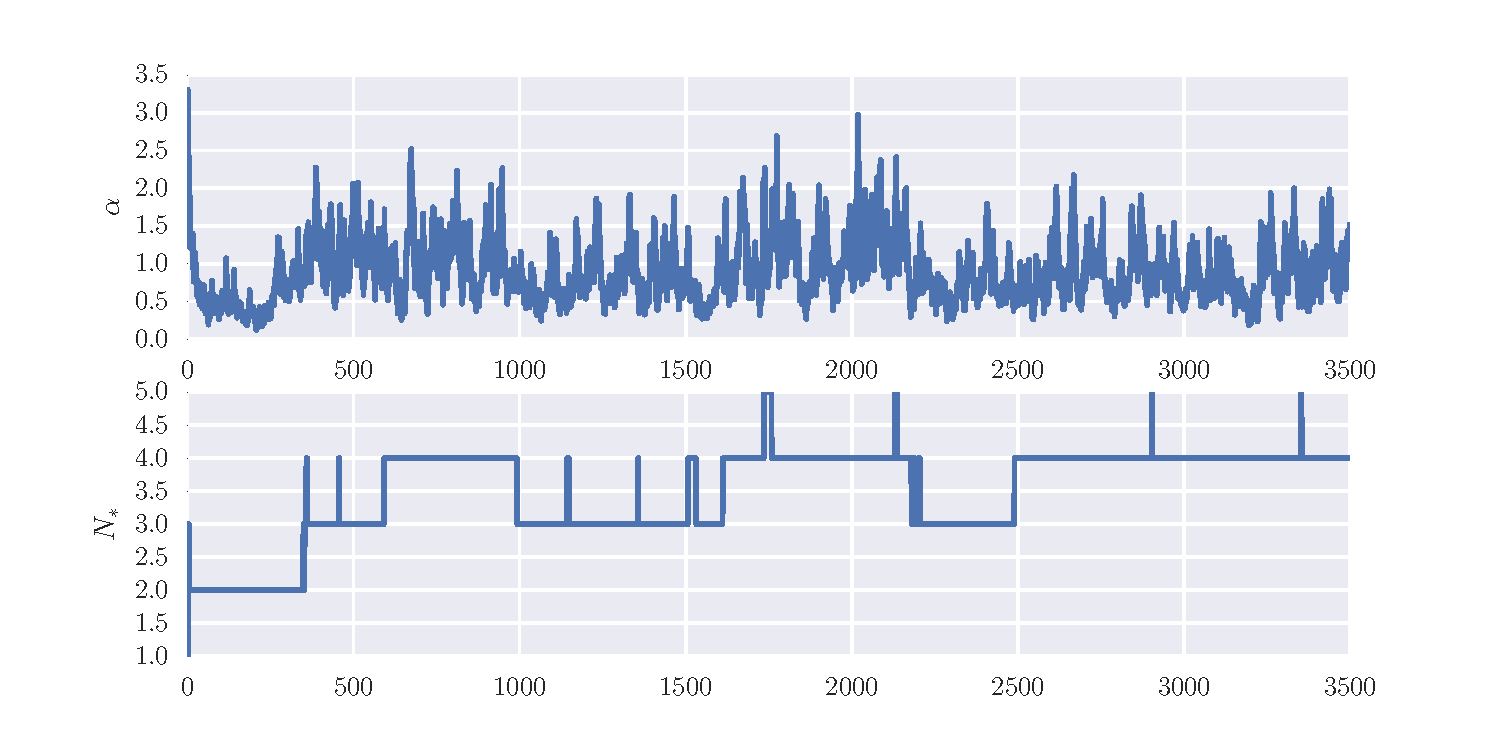
\includegraphics[width=\textwidth]{n3115_traces.pdf}
\caption{Trace plots for $\alpha$ (top) and $n_*$ (bottom), indicating the mixing of the chain.}
\label{n3115_trace}
\end{figure}

\begin{figure}
\centering
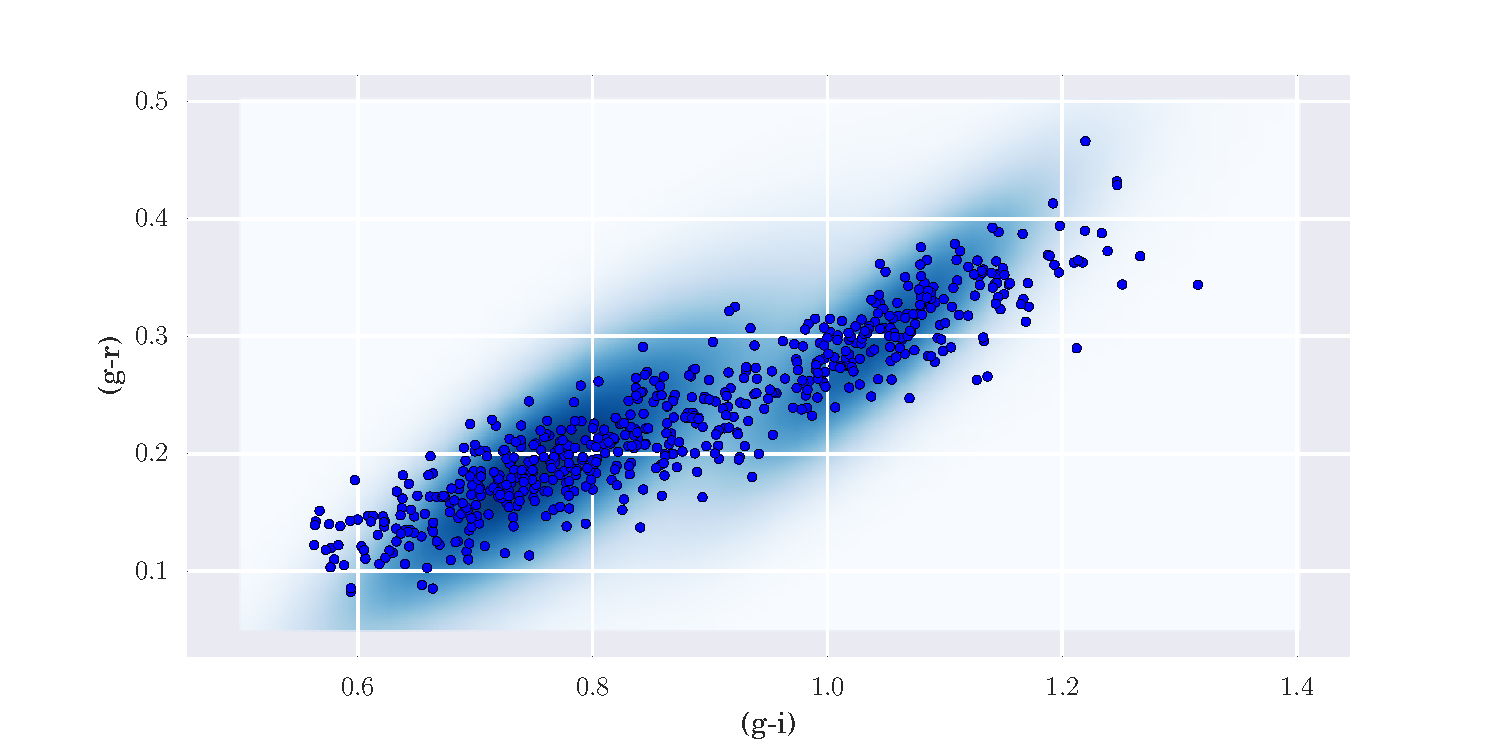
\includegraphics[width=\textwidth]{n3115_data_fit.pdf}
\caption{Plot of the mean functional for NGC 3115 overlaid on the scatter plot for data. While shapes of the model
don't appear to do the best job capturing the data, the bimodal structure is clearly captured and the locations
appear to match well.}
\label{n3115_functional}
\end{figure}

\begin{figure}
\centering
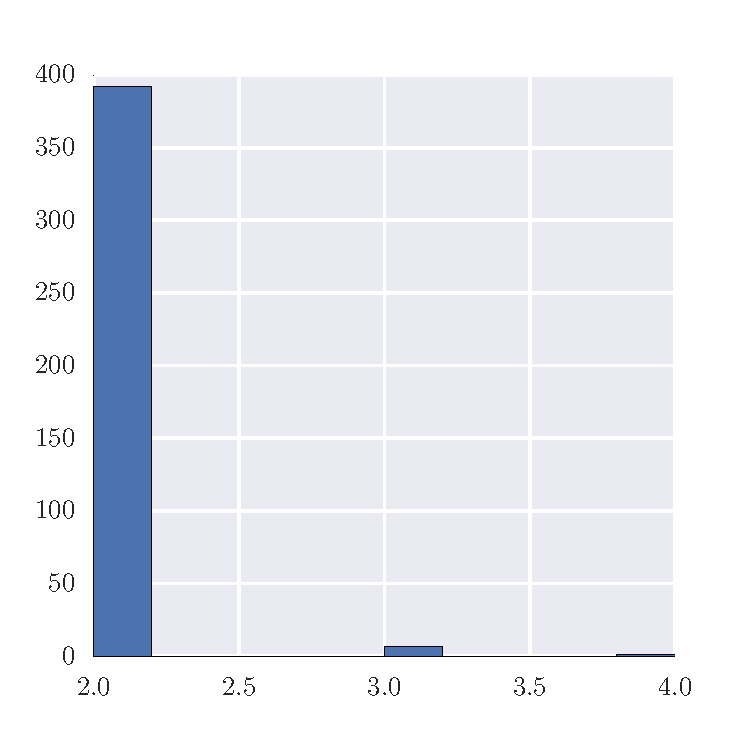
\includegraphics[width=0.7\textwidth]{n3115_mode_post.pdf}
\caption{Histogram of the modes recovered for 400 realizations of the G function
using the mode finding method. The underlying distribution appears to be bimodal with high probability.}
\label{n3115_modes}
\end{figure}

\subsection{NGC4494 Photometry}
NGC 4494 is a similar-sized galaxy to NGC 3115, located slightly farther away and with a more spherical morphology.
NGC 4494 can be thought of essentially as a round ball of stars, whereas NGC 3115 is more football-shaped.
The dataset I am using was published in \citealt{foster2011}, and features around 450 GCs.

Unlike NGC 3115, NGC 4494 is not generally thought of as a good case of bimodality. The distribution is less clear in
this regard,
and indeed NGC 4494 stands out as somewhat of an outlier among extragalactic GC studies which examine relative
fractions of red and blue colored GCs. 

I plot the color-color distribution of NGC4494 in Fig.~\ref{n4494_data}. I applied the model above and ran it for
3000 steps, discarding the first 1000 and thinning by a factor of 5.
In Fig.~\ref{n4494_trace}, I plot trace plots for $\alpha$ and $n_*$.

In Fig.~\ref{n4494_functional}, I plot the mean inference for 400 realizations
of $G$ from the blocked Gibbs sampler. In Fig.~\ref{n4494_modes}, I plot the histogram of modes found in NGC 4494
from my mode-finding algorithm. Both the mode-finding algorithm and the actual plot of the functional seem to highly
favor a unimodal case. This could perhaps suggest that NGC 4494 only had a single epoch of formation for its GC system,
or, more likely, it's assembly has been more continuous, without the two distinct epochs of NGC 3115.

\begin{figure}
\centering
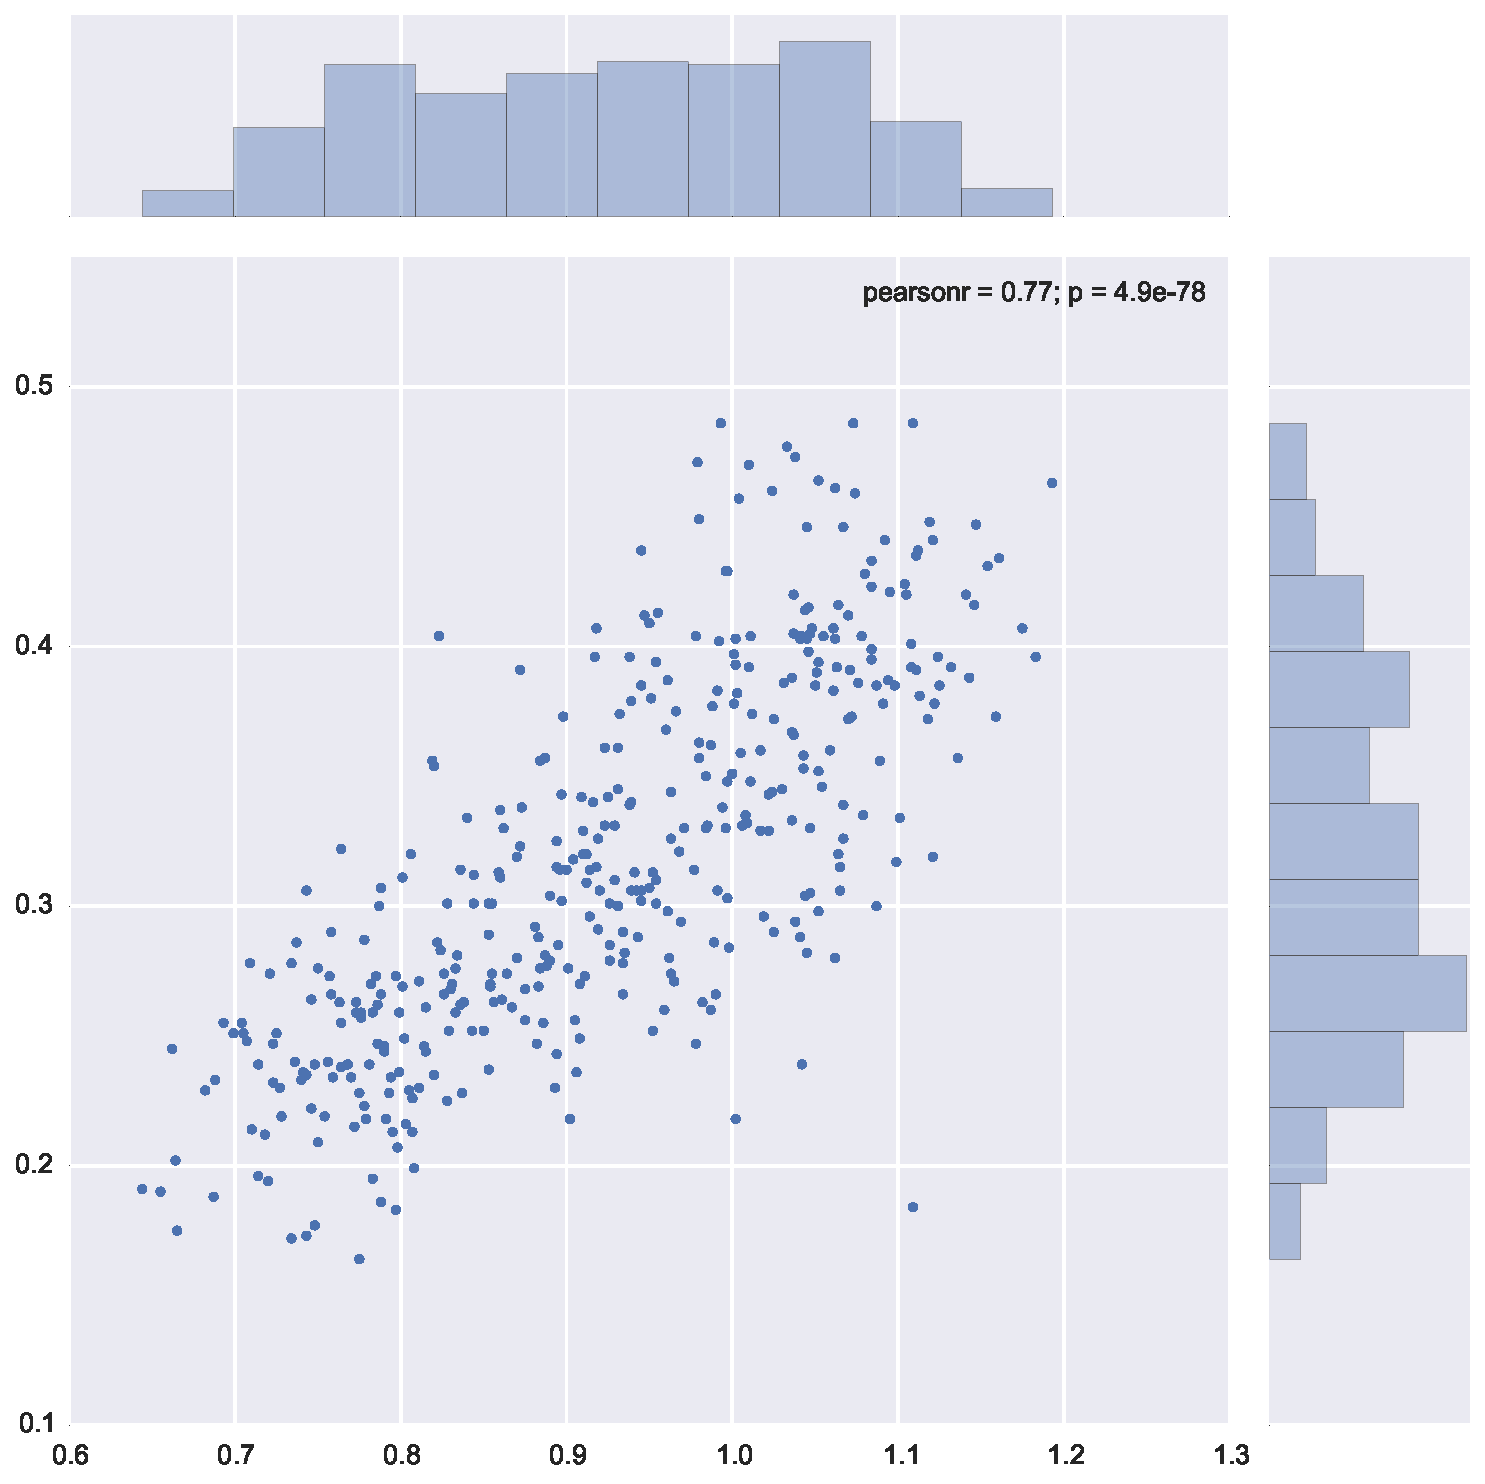
\includegraphics[width=0.6\textwidth]{n4494_data.pdf}
\caption{$(g-i)$ vs.~$(r-i)$ color-color plot of selected GCs around NGC 4494. The bimodal structure is less clear, although
perhaps one could imagine the top histogram contains some such structure.}
\label{n4494_data}
\end{figure}

\begin{figure}
\centering
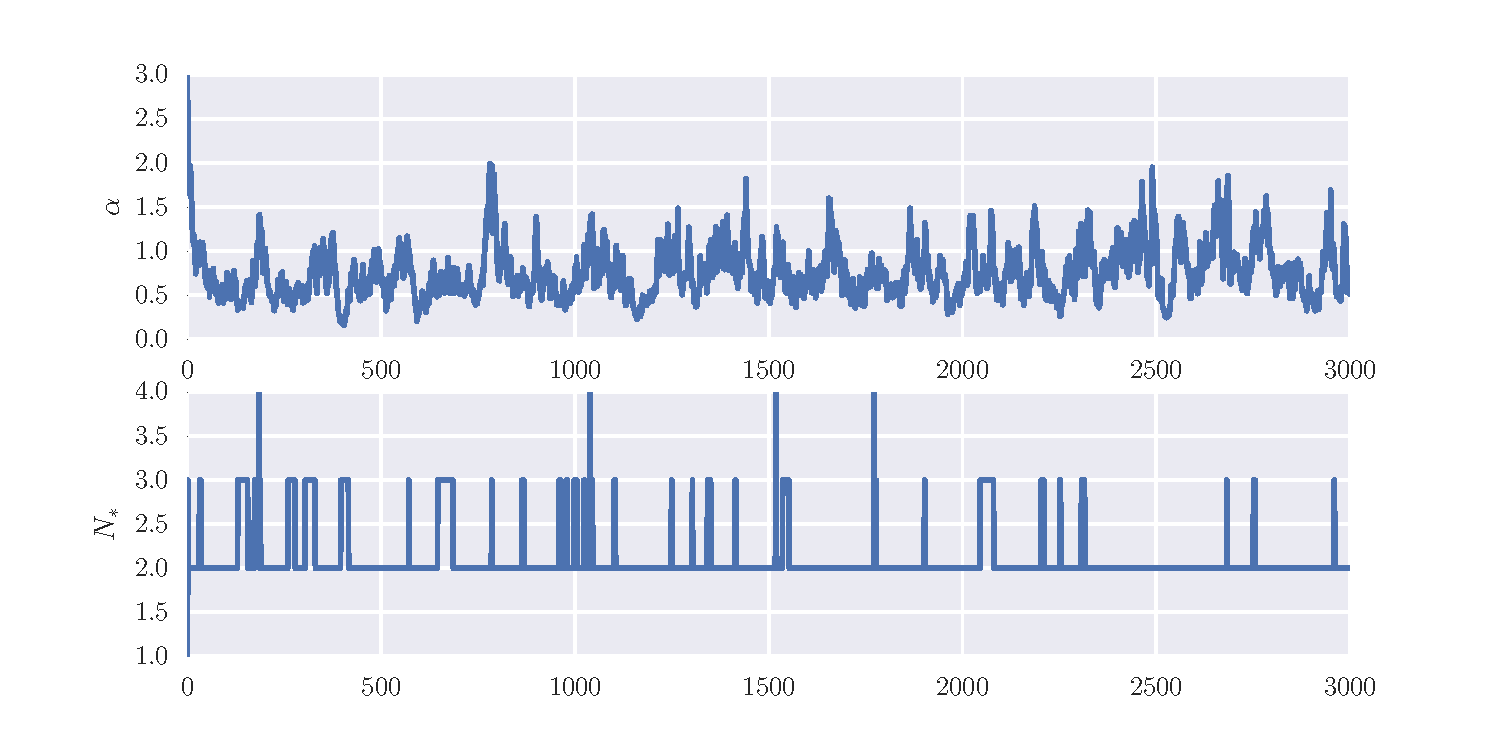
\includegraphics[width=\textwidth]{n4494_traces.pdf}
\caption{Trace plots for $\alpha$ (top) and $n_*$ (bottom), indicating the mixing of the chain. The model
clearly wants fewer populations to fit this distribution than were required for NGC 3115.}
\label{n4494_trace}
\end{figure}

\begin{figure}
\centering
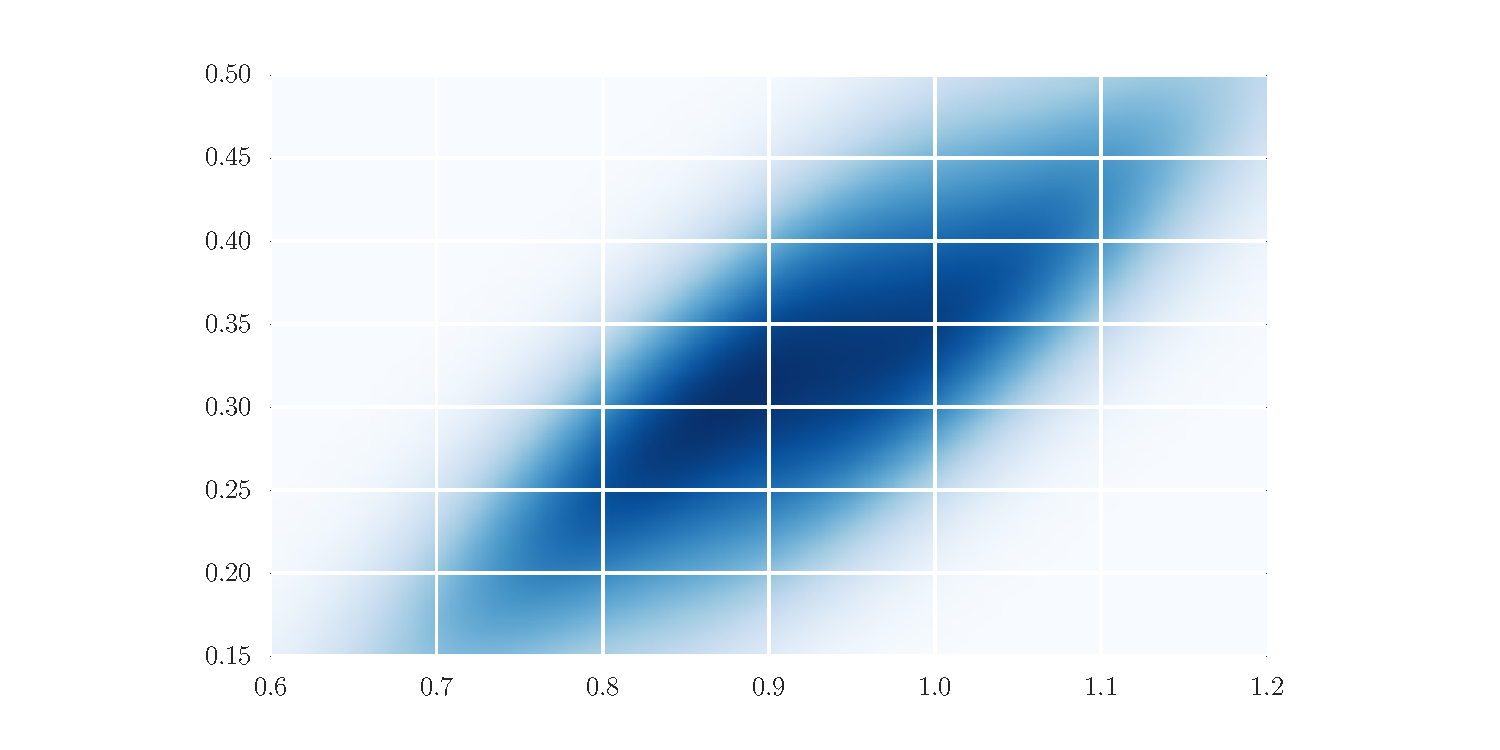
\includegraphics[width=\textwidth]{n4494_data_fit}
\caption{Plot of the mean functional for NGC 4494 overlaid on the scatter plot for data. These data do not appear
to display any clear multi-modality, instead seeming to be modeled reasonably by a single continuous population.}
\label{n4494_functional}
\end{figure}

\begin{figure}
\centering
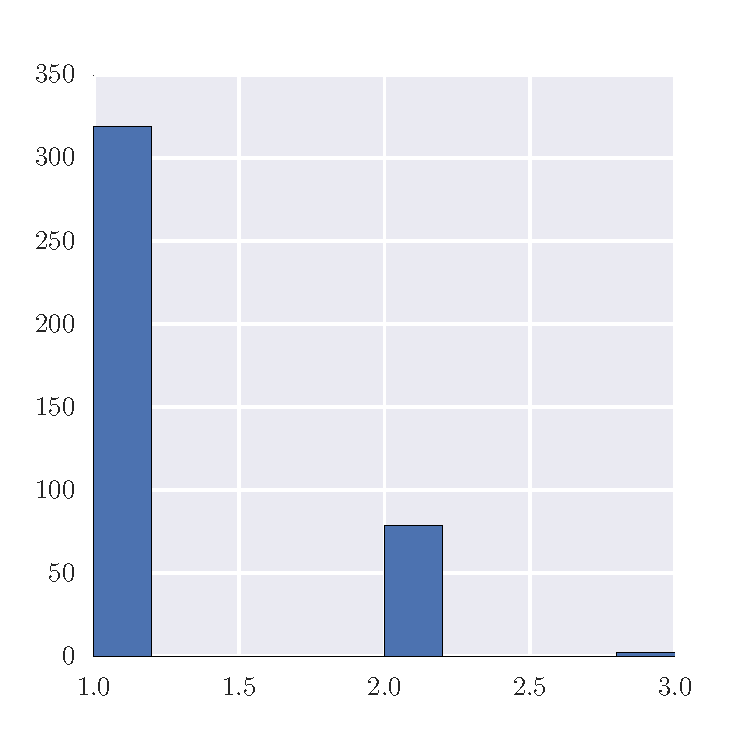
\includegraphics[width=0.7\textwidth]{n4494_mode_post.pdf}
\caption{Histogram of the modes recovered for 400 realizations of the G function
using the mode finding method for NGC 4494. The underlying distribution appears to be unimodal with high probability,
although clearly some of the realizations do have a second mode.}
\label{n4494_modes}
\end{figure}

\section{AREAS FOR FURTHER STUDY}
I think the model is currently weakest in its treatment of the covariance matrix, $\Sigma$.
The shapes inferred for the distributions appear to be off for some of the data, and the inferences appear to be
sensitive to prior specification for $\Sigma$ specifically. I think allowing the $\Sigma$ to vary as for each
kernel will be a big improvement on the model. I already added this change to the code, but I didn't have a chance to
optimize the code correctly, and the current way I have coded it makes it very inefficient for MCMC sampling. I believe
this would make a big improvement to the model.

Once this is specified, one could play around with several model expansions. For one, the assumption of multivariate
normals can be relaxed, and a natural extension would be to multivariate-t distributions. This would potentially
allow the tails of the distributions to be better modeled, perhaps making the $n_*$ values more meaningful.
Related to this is expanding the Dirichlet process to include other distributions, such as a 2-parameter beta process
or a more general Pitman-Yor process \citep{ishwaran2001}. Such an extension plugs in nicely to the
blocked Gibbs sampler without too much more effort. Both of these expansions could also
have the effect of offering more control over the clustering of the data, again possibly making the $n_*$ values meaningful.
Indeed, I had originally planned on implementing one or both of these processes. However, once it became clear to me that
requiring the same $\Sigma$ across the clusters was having an effect on the model, that became my primary focus as I was
unsure the exact clustering could be trusted much in the current model. 

In addition to areas of improvement in the model, one could also look into making more inferences about the populations
themselves. For example, it is of astrophysical interest what the relative fractions of red and blue globular clusters are
in galaxies well-modeled by two distributions. Typically, uncertainty about the underlying functional
form of the distributions is not folded in to any sort of inference on this quantity. Once one has realizations from
the non-parametric functional, one could create posterior predictive datasets and perform similar analysis to
identify the uncertainty in such a quantity. In addition the relative locations of the different populations in color-color
space is also of interest, as these may indicate the degree of enrichment of different populations. Both quantities
can be derived from the MCMC simulations in a straightforward manner once the simulations have been carried out.

Application of this method to other galaxies is also of interest. Many galaxies which are accepted as being
bimodal are not as clearly so as NGC 3115, and there are other outliers such as NGC 4494 which would be interesting
to test. Once the model is improved and refined further, application to a larger dataset would be a useful exercise.
%\bibliographystyle{apj}
%\bibliography{bibtex_n3115.bib}

\begin{thebibliography}{}
\expandafter\ifx\csname natexlab\endcsname\relax\def\natexlab#1{#1}\fi

\bibitem[{{Brodie} \& {Strader}(2006)}]{brodie2006}
{Brodie}, J.~P., \& {Strader}, J. 2006, ARAA, 44, 193

\bibitem[{{Brodie} {et~al.}(2012){Brodie}, {Usher}, {Conroy}, {Strader},
  {Arnold}, {Forbes}, \& {Romanowsky}}]{brodie2012}
{Brodie}, J.~P., {Usher}, C., {Conroy}, C., {et~al.} 2012, ApJL, 759, L33

\bibitem[{{Foster} {et~al.}(2011){Foster}, {Spitler}, {Romanowsky}, {Forbes},
  {Pota}, {Bekki}, {Strader}, {Proctor}, {Arnold}, \& {Brodie}}]{foster2011}
{Foster}, C., {Spitler}, L.~R., {Romanowsky}, A.~J., {et~al.} 2011, MNRAS,
  415, 3393

\bibitem[{Ishwaran \& James(2001)}]{ishwaran2001}
Ishwaran, H., \& James, L.~F. 2001, JASA, 96, 161

\bibitem[{{Jennings} {et~al.}(2014){Jennings}, {Strader}, {Romanowsky},
  {Brodie}, {Arnold}, {Lin}, {Irwin}, {Sivakoff}, \& {Wong}}]{jennings2014}
{Jennings}, Z.~G., {Strader}, J., {Romanowsky}, A.~J., {et~al.} 2014, AJ, 148,
  32

\bibitem[{{Zepf} \& {Ashman}(1993)}]{zepf1993}
{Zepf}, S.~E., \& {Ashman}, K.~M. 1993, MNRAS, 264, 611

\end{thebibliography}

\end{document}












